\chapter{آشنایی با پروژه}

\begin{figure}[h]
    \centering
    
\includegraphics[width=0.7\textwidth]{./1-Introduction/yarcee.png}
    \caption{لوگو پروژه}
    \label{fig:yarcee}
\end{figure}

YARCEE مخفف
\lr{Yet Another Remote Code Execution Engine}
یک سرویس ابری اجرای کد می‌باشد.
معماری این پروژه مایکروسرویس است و سرویس ها با زبان Go نوشته شده اند.
برخی از ویژگی های کلیدی پروژه شامل:

\begin{itemize}
    \item اجرای کد زبان های مختلف مانند python - nodejs - c - c++ و ...
    \item عدم دسترسی پروژه ها به یکدیگر به دلیل اجرا در micro-vm
    \item ادیتور انلاین و ویرایش در مرورگر
    \item قابلیت ساخت ، ادامه و تغییر نام پروژه
    \item همروند بودن اجرای کد توسط صف پیام RabbitMQ
\end{itemize}


\newpage

این پروژه یک سرویس ابری است که شامل ویژگی های یک محصول واقعی است. کاربر امکان ثبت نام و ورود دارد.
می‌تواند پروژه جدید بسازد و آن را ویرایش و حذف بکند.
در فصل جمع بندی نگاهی به آینده این محصول می‌کنیم اما قبل از آن به صورت خیلی خلاصه نحوه عملکرد این سیستم را بررسی می‌کنیم.


\begin{figure}[htbp]
    \centering
    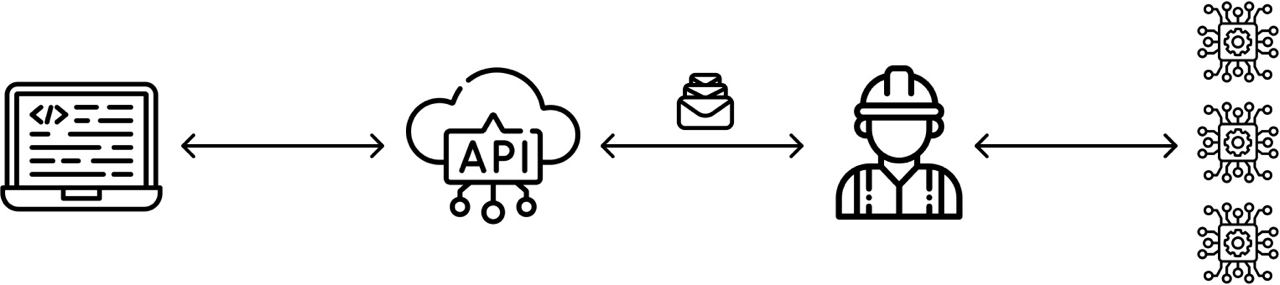
\includegraphics[width=0.7\textwidth]{./1-Introduction/overview.jpg}
    \caption{ساختار کلی پروژه}
    \label{fig:yarcee-overview}
\end{figure}

پس از ثبت نام و ورود به داشبورد، از قالب های از پیش تعریف شده یکی را به دلخواه انتخاب می‌کنیم. هر قالب شامل اسمی تصادفی، کد اولیه زبان و اطلاعاتی در مورد اجرای آن می‌باشد.
پس از ویرایش کد آن را اجرا می‌کنیم.

در پشت صحنه درخواستی برای دریافت خروجی کد به سرویس API زده می‌شود. وظیفه این سرویس ارتباط مستقیم با پایگاه داده و گوش دادن به وضعیت اجرای کد و خروجی آن می‌باشد.


این درخواست روی صف RabbitMQ ارسال می‌شود و توسط سرویسی از صف دریافت می‌شود.
این سرویس سپس درخواست را برای پردازش یکی از vm هایی که در حالت آماده باش قرار دارد می‌فرستد و خروجی اجرای کد را دریافت می‌کند.

مجموعه از vm ها در حالت آماده باش قرار دارند که پس از اجرای کد حذف و سپس جایگزین به مجموعه اضافه می‌شود.
متصل به هر vm فایل سیستمی از پیش ساخته شده که است که باینری کامپایلرهای مختلف درون آن وجود دارد.


وابستگی اصلی این پروژه به Firecracker می‌باشد که برای مدیریت micro-vm ها به کار می‌رود.
برای ارتباط با این ابزار از sdk زبان GO آن استفاده شده است.
از مزیت های استفاده از روش micro-vm می‌توان سرعت بسیار بالاتر نسبت به vm اشاره کرد.
همچنین این روش امنیت بالاتری نسبت به اجرای کد در محیط های کانتیری مانند docker دارد زیرا micro-vm ها به طور کل از یکدیگر جدا هستند.

بخش مهم دیگر این پروژه محیط وب و ادیتور انلاین آن می‌باشد. کلاینت با زبان TypeScript نوشته شده است و از فریمورک Next.js استفاده می‌کند.
کتابخانه ui زبان به طبع React می‌باشد.
در بخش ادیتور امکان ویرایش کن و درخواست اجرا وجود دارد. با فشردن اجرا کلاینت هر از ۱۰۰ میلی ثانیه به سرور درخواست میزد تا خروجی کد درخواست شده را دریافت کند. پس دریافت stdout و stderr این چرخه را متوقف می‌کند.

در ادامه به معرفی هر سرویس خواهیم پرداخت.